\chapter{Konzeption}

Bei der Konzeption der eigenen Android-App liegt der Fokus auf der Erfüllung aller in Kapitel 4 als relevant klassifizierten Kriterien.
Hierzu werden im Folgenden Implementierungsansätze vorgestellt, die für einen ersten Prototypen umgesetzt werden sollen.

\section{Sichtbarkeit des Systemzustandes}
Um dem Benutzer zu jeder Zeit einen Überblick über die App zu ermöglichen, wird eine Statusleiste, wie sie in Kapitel 4 bei allen drei Apps vorhanden war, eingesetzt.
Diese soll einerseits den aktuellen Modus anzeigen, andererseits soll erkenntbar sein, welche Aktionen in dem aktuellen Systemzustand ausführbar sind, und welche nicht.

\section{Fehlervorbeugung}
Zusätzlich soll das Deaktivieren von nicht-ausführbaren Aktionen dafür sorgen, dass Situationen, in denen Fehler entstehen können, präventiv vermieden werden.

\section{Benutzerkontrolle und -freieht}
Gerade die fehlende Undo/Redo-Funktionalität hat sich bei den beiden Apps \pm{} und \ms{} als signifikantes Usability-Problem identifizieren lassen.
In der App soll diese Funktionalität über zwei dedizierte Icons in der Menübar angeboten werden.

\section{Konsistenz und Standards}
Um eine positive Benutzererfahrung zu generieren, und die Benutzung von nicht-intuitiven Icons oder Patterns zu vermeiden, werden bei der Implementierung die Design-Richtlinien von Google befolgt.
Diese bieten sowohl Konzepte zur Umsetzung verschiedener UI-Elemente, als auch eine Vielzahl konsistent gestalteter Icons an. 

\section{Wiedererkennung statt Erinnern}
Eine minimierte kongnitive Belastung soll durch die Verwedung von gleichen Icons für gleiche Aktionen erzielt werden.
So soll im ``Zeichen-Modus'' als auch im ``Text-Modus'' ein Mülleimer-Icon in der Menüleiste die Möglichkeit bieten, die markierte Form bzw. den ausgewählten Text zu löschen.

\section{Fleixibilität und Effizienz der Benutzung}
Der Benutzer soll in der Lage sein, die gezeichneten Formen im Nachhinein zu bearbeiten.
Hierzu soll es die Möglichkeit geben, dass der Benutzer bereits zu Begin eine Standard-Farbe festlegen kann, in der alle nachfolgenden Formen gefärbt werden, oder einzelne Formen nachträglich umfärben kann.
Außerdem soll es für den erfahrenen Benutzer Abkürzungen für Aktionen wie das Eintragen von Texten geben.
Dies kann durch eine Lang-Klick Aktion auf die gewünschte Form gelöst werden.

\section{Erkennbarkeit, Diagnose und Erholung von Fehlern}
Zunächst liegt das Ziel fehleranfällige Sitationen präventiv zu vermeiden.
Sollte es dennoch zu einem Fehler kommen, soll eine kurze, aber informative Nachricht in Form eines ``Toast'' auf dem Bildschirm angezeigt werden.
Zu keiner Zeit sollte der Benutzer in eine endlose Spirale von Fehlerzuständen gelangen können, welche er nur durch das Beenden oder die Deinstallation der App verlassen kann.

\section{Hilfe und Dokumentation}
Wie in Kapitel 4 festgestellt, ist die Verwendung eines Hilfe-Overlays sinnvoll.
Dieses soll zum initialen Start der App den Benutzer über die verschiedenen Modi informieren.
Beim jeweils ersten Wechsel in einen Modus soll ein weiteres Hilfe-Overlay angezeigt werden, welches die verschiedenen Aktionen des ausgewählten Modus vorstellt.
\todo{Tap Taget}

\section{Adäquater Umgang mit Unterbrechungen}
Die App soll bei Unterbrechung der Aktivität wie der Navigation zu einer anderen App, oder dem Wechseln auf den Home-Bildschirm alle Informationen speichern, und beim Zurückkehren in die pausierte App wieder anzeigen.
Dies kann durch die Implementierung eines \emph{Saved States} erzielt werden.
\todo{Saved State}

\section{Fokussieren der Informationen}
Ein weiterer Wichtiger Umsetzungspunkt liegt beim Hervorheben wichtiger Informationen auf dem Bildschirm.
So sollen markierte Formen durch die Benutzung einer Akzent-Farbe hervorgehoben werden.
\todo{Accent-Color}

\section{``Joy of Use''}
Die Bedienung der App soll intuitiv und einfach sein, um ein positives Nutzungerlebnis zu garantieren.
Hierzu sollen verschiedene Gesten zur Navigation im Bild genutzt werden.
\todo{Gesture Support}

\section{Unterstützung verschiedener Bildschirmausrichtungen}
Insbesondere aufgrund des Zeichen-Fearues sollte die App im Querformat genau so einfach zu bedienen sein, wie im Hochformat.
So bietet sich dem Benutzer nämlich die Möglichkeit im Hochformat aufgenommene Bilder auch in diesem zu Bearbeiten.
Dies hat den Vorteil, dass das Bild in seinem ursprünglichen Seitenverhältnis angesehen und bearbeitet werden kann, und nicht in ein falsches erst skaliert werden muss.

\section{Ergenomische Gestaltung der physischen Interatkion}
\todo{Hier noch was finden, was anders als Joy of Use ist}

\section{Einfache Eingabe, Bildschirmlesbarkeit und Übersichtlichkeit}
Der Benutzer soll in der Lage sein, die gesamte App mit einer Hand bedienen zu können.
Hierzu müssen neben dem Pinch-2-Zoom auch noch Doppel-Tap Gesten verarbeitet werden können.
Außerdem sollen Formen durch eine natürliche Drag-Geste mit einem Finger verschoben oder vergrößert werden können.

\section{Vorgehensweise bei Implementierung eigener Software-Lösung}
\todo{Alle Aussagen mit Zitaten belegen?}
\todo{Schreiben was ich in dieser section mache}
\todo{Bezug auf Ergebnisse von alternativen} 
\subsection{Die 8 Goldenen Regeln von Shneiderman}

\citeauthor{Shneiderman04} definieren in ihrem Buch ``Designing the User Interface: Strategies for Effective Human-Computer Interaction'' die sogenannten ``8 Goldenen Regeln des Interface Designs''.  Die acht Regeln lauten wie folgt:

\begin{enumerate}
  \item Bemühe Dich um Konsistenz (``Strive for consistency'')
  \item Erlaube erfahrenen Benutzern die Nutzung von Abkürzungen (``Enable fequent users to use shortcuts'')
  \item Biete informative Rückkopplung (``Offer informative feedback'')
  \item Biete ein klares Ende von Teildialogen an (``Design dialogs to yield closure'')
  \item Biete Fehlervermeidung und einfache Fehlerbehandlung an (``Offer error protection and simple error handling'')
  \item \label{itm:undo} Erlaube eine einfach Rücknahme von Aktionen (``Permit easy reversal of actions'')
  \item Gib dem Benutzer die Kontrolle (``Support internal locus of control'')
  \item Minimiere Gedächtnisbelastung (``Reduce short-memory load'')
\end{enumerate} 

Diese Regeln sind ein weiterer guter Anhaltspunkt für die Entwicklung einer guten Software-Lösung, die den Faktor der Usability mit berücksichtigt. Vor allem der Punkt \autoref{itm:undo} sollte bei einer Applikation, deren Fokus auf den aneinander gereihten Aktionen des Benutzers beruht, erfüllt sein. Dies soll durch einen Undo- bzw. Redo-Button in der oberen Menüleiste gewährleistet werden. \\

Die Konsistenz der Applikation soll durch die Benutzung der \citet{AndroidMG} gewährleistet werden. 
So werden einerseits nur Icons aus der Standard Google-Library verwendet, andererseits werden diverese Guidelines die auf \citet{AndroidMG} vorgestellt werden, benutzt. 
Hierzu zählt auch die sogenannte \emph{Feature-Discovery}.
Dabei soll der Benutzer durch ein hinweisendes Overlay dazu aufgefordert werden, gewisse Funktionen der App zu erkunden. 
Dies ist besonders bei einer App, in der es mehr als eine zentrale Funktion gibt, hilfreich und wichtig. \\

\begin{figure}[h]
  \centering
  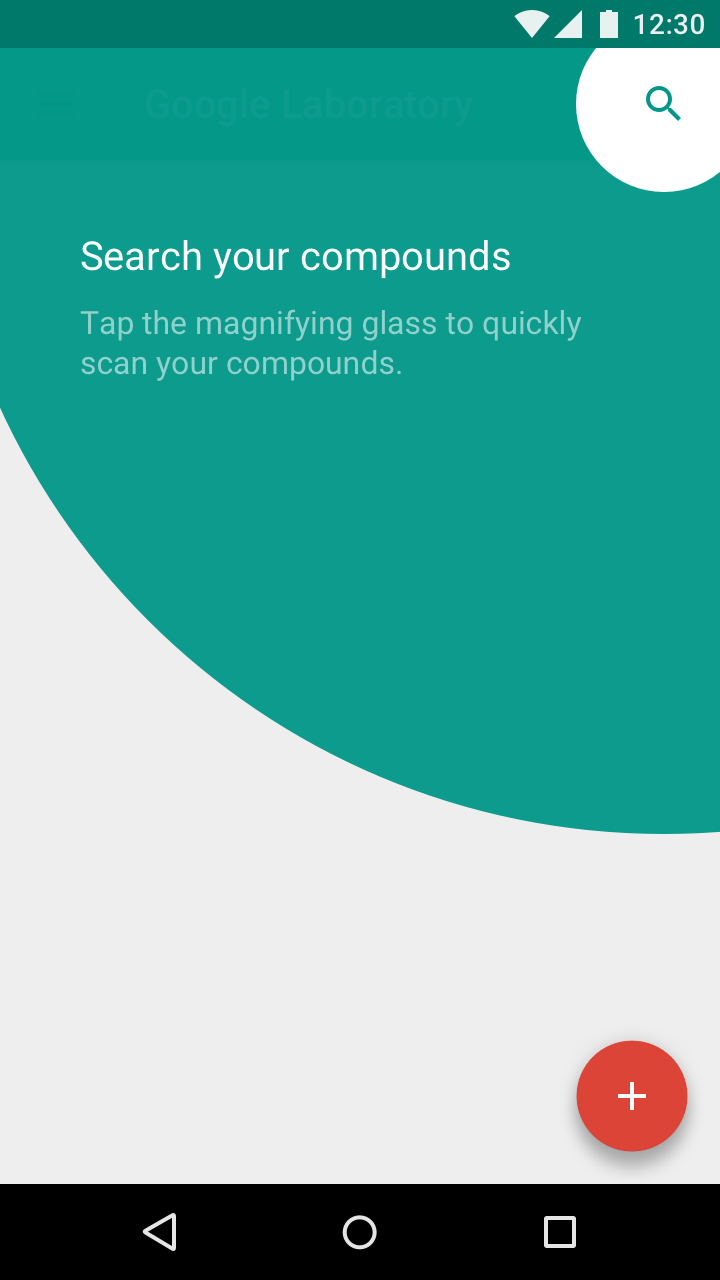
\includegraphics[keepaspectratio, width=0.5\textwidth]{fd}
  \caption{Feature-Discovery in Form eines Tap-Targets}
  \label{fig:fd}
\end{figure}

In \autoref{fig:fd} sieht man eine beispielhafte Implementierung einer solchen Feature-Discovery in Form eines Tap-Targets.
Hierbei wird der Benutzer durch eine Hervorhebung bestimmter UI-Elemente auf Funktionen hingewiesen. 
Zusätzlich wird ein kurzer erklärender Satz mit einem zusammenfassenden Titel angezeigt. \\

\subsection{Gesture-Support}

Mit der Einführung Applikationen für mobile Endgeräte hat sich ein weiteres, vorher nicht relevantes, Usability-Problem etabliert: 
\emph{Die geringe Größe des Bildschirm}. \\

Die relativ kleine physikalische Größe der Smartphone-Displays bringt verschiedene Probleme mit sich. 
So muss einerseits die Funktionalität einer ganzen Desktop-Applikation auf ein viel kleineres Display passen, ohne den Content zu verändern, oder gar unleserlich zu machen.
Andererseits muss dem Benutzer eine intuitive und effiziente Navigationsmöglichkeit gegeben sein, um zwischen verschiedenen Inhalten zu wechseln. \\

Hierzu schreiben \citeauthor{Gutwin04}, dass die Navigationen auf kleinen Bildschirmen selbst im besten Fall deutlich langsamer sei als auf normal-großen Bildschirmen.
Sie führen weiter an, dass eine Übersicht über den gesamten Systemzustand wertvoll sei, da dies dem Nutzer eine schnellere Navigation erlaube. \\
Nach \citeauthor{Gutwin04} eigne sich die Technik des ``Two-Level Zooms'' besonders gut für Navigationsaufgaben, wohingegen Panning-Strategien eher negativ von den Test-Personen aufgenommen worden seien \citep[Seite 8]{Gutwin04}.  

\todo{Tap-Target prompts}

\subsection{Iterativer Entwicklungsprozess}
3 Iterationen jeweils Mitte Dezember, Januar und Februar \\
Feedback in Form von Gitlab-Issues und Beobachten von Testpersonen (Usability-Experimente) \\
1. Iteration (Dezember): App mit floating buttons (screenshots vorher-nachher)
2. Iteration (Januar): App mit status bar (screenshots vorher-nachher)
3. Iteration (Februar): App mit Help-Overlay \& verbesserter Statusbar (screenshots vorher-nachher)
\subsection{DIN und ISO-Normen}
\subsection{Material Design-Guidelines}
\subsection{ABC-Modell}
\subsection{Gesture-Support (papers)}
Zoom-Area und Panning am besten geeignet um Content auf kleinen Displays darzustellen \\

